\documentclass{erdc}
\usepackage{amssymb}
\usepackage{url}
\begin{document}

\frontmatter

%\laboratory{Information Technology Laboratory}

% Assigned report number goes here. The CRREL sample number is not this report.
\reportnum{ERDC/ITL TR-XX-XX}

\program{Engineered Resilient Systems}

\title{Quantum and Hybrid-Quantum Physics-Informed Neural Networks for Shallow-Water Flows}

\subtitle{}

\date{October 2026}

\author{Corey~Trahan \and Mark~Loveland \and Samuel~Dent}

\affiliation{Information Technology Laboratory\\
  U.S. Army Engineer Research and Development Center\\
  3909 Halls Ferry Road\\
  Vicksburg, MS 39180}

\coverart{nola}

\reporttype{Final Report}

% \distribution{Distribution authorized to U.S. Government Agencies
% only; Test and Evaluation; November 2005.  Other requests should be
% referred to U.S. Army Engineer Research and Development Center}

%\additionalinfo{}

\begin{abstract}
This report describes a controlled comparison of classical,
hybrid-quantum, and full-quantum physics-informed neural networks for
the shallow-water equations. The three families share one trainer, one
strong-form residual loss, and one hyperparameter-search protocol. They
differ in the network that represents the flow. The classical family
assigns each field its own multilayer perceptron. The hybrid-quantum
family keeps that perceptron and adds a residual quantum circuit on
each tower. The full-quantum family has no hidden perceptron: each
field is a linear readout of a variational circuit applied to the
coordinates, together with the classical encoder that feeds the
circuit. Every circuit is evaluated by noiseless statevector
simulation.

The comparison is presented on three shallow-water problems: a
frictional linear tide, a wet-bed dam break, and a two-dimensional
steady eddy lattice. Each study ranks completed trials by the
physics-informed scoring loss alone. On the tide, the lowest loss is a
428-parameter hybrid model, and a retraining of that architecture
follows the analytic wave, with relative \(L_2\) errors of \(2.9\%\) in
elevation and \(7.5\%\) in velocity. On the dam break, classical models
hold most of the loss--parameter front, and the best hybrid loss is
about \(10\%\) below the best classical loss. The equation residuals of
those two models are nearly the same, and the retrained hybrid smooths
the shock and the rarefaction, consistent with earlier reports that
quantum networks handle shocks poorly~\cite{leong2025highspeed}. On the eddy lattice, hybrid models reach
the lowest losses, but the retrained hybrid has relative \(L_2\) errors
of \(1.3\%\) in depth and \(121\%\) and \(130\%\) in the two velocity
components. The circuits are noiseless statevector
simulations, so these differences are differences of representation.
\end{abstract}

%\disclaimer{Some other disclaimer}

%\preparedfor{U.S. Army Engineer Research and Development Center\\
%  3909 Halls Ferry Road, Vicksburg, MS 39180-6199}

%\contractnum{}

\monitoredby{U.S. Army Engineer Research and Development Center\\
  3909 Halls Ferry Road, Vicksburg, MS 39180-6199}

%\preparedfor{}

\maketitle

\tableofcontents

\listoffiguresandtables

\chapter{Preface}
This technical report documents a software framework and an experimental
protocol for comparing physics-informed neural networks (PINNs), hybrid
quantum physics-informed neural networks, and full-quantum
physics-informed networks on the shallow-water equations. The
comparison uses one trainer and three benchmarks: a smooth linear tide,
a dam-break shock, and a two-dimensional steady eddy lattice. The quantity of interest is
representational performance: physics-informed loss, agreement with a
reference solution, and the number of trainable parameters. The quantum
circuits are simulated. The report does not claim a quantum
computational advantage.

This investigation was conducted by the U.S. Army Engineer Research and
Development Center (ERDC), Information Technology Laboratory (ITL), as
part of the Engineered Resilient Systems (ERS) fundamental research
program. The work was performed to investigate emerging
quantum--classical computational approaches for physics-informed
machine learning and their potential applicability to computational
science and engineering problems of interest to ERDC and the U.S. Army
Corps of Engineers. The work was performed under the general direction
of Dr.~Robert D. Moser, Director, Information Technology Laboratory,
ERDC. At the time of publication of this report, Dr.~Beth Fleming was
Director of ERDC, and LTC Joshua Haynes was Commander of ERDC.

\mainmatter

\chapter{Introduction}
\label{sec:introduction}

Physics-informed neural networks (PINNs) approximate solutions of ordinary
and partial differential equations by representing the solution with a
differentiable network and penalizing violations of the governing
equations, initial and boundary conditions, and available observations
\cite{Raissi2019}. This formulation is flexible, but its practical
performance depends on how well the network represents the solution and
how effectively the optimizer balances the competing terms in the loss.
Accuracy and convergence can therefore vary with architecture,
initialization, loss weights, collocation strategy, and the structure of
the target field. A low physics residual does not, by itself, guarantee
small error against a reference solution. These sensitivities matter
especially when comparing smooth solutions with shocks or multiple
spatial scales.

This motivates investigating alternative function representations within
the same physics-informed framework. Parameterized quantum circuits
provide one such representation: encoded inputs act on a multi-qubit
state, and circuit expectation values can be differentiated and trained
against differential-equation residuals. Entangling gates can couple
information across qubits, providing a possible mechanism for representing
interactions among encoded input features in the map from spatial and
temporal coordinates to a predicted field. The circuit's representational
capacity depends not only on its parameter count, but also on its input
encoding, entangling structure, depth, and measured observables.
Expressibility and entangling capability are distinct descriptors of a
circuit ansatz \cite{Sim2019}; neither alone guarantees accurate
approximation of a particular PDE solution or efficient training. Quantum
circuits are therefore worth investigating as alternative representations,
but their use does not by itself establish an advantage on quantum
hardware, where input encoding, measurement, circuit depth, and noise also
affect cost and reliability.

Kyriienko, Paine, and Elfving represented solutions of nonlinear
differential equations by expectation values of differentiable quantum
circuits and minimized the resulting residuals, including for a nozzle
flow \cite{Kyriienko2021}. Markidis examined a continuous-variable quantum
PINN for the one-dimensional Poisson equation and the roles of
optimization, residual formulation, and depth \cite{markidis2022physics}.
Vadyala and Betgeri combined classical and quantum processing in one
physics-informed implementation \cite{vadyala2023general}. Later work has
considered fluid equations and hybrid layouts. Sedykh and coauthors placed
a variational circuit beside a classical perceptron for steady laminar
flow in a three-dimensional mixer \cite{Sedykh2024}. Trahan, Loveland,
and Dent compared classical, hybrid, and fully quantum networks on a
spring-mass oscillator, the Poisson equation, and viscous Burgers'
equation. They found that error varied with qubit count, variational
depth, and the placement of the quantum node, as well as with the model
class \cite{Trahan2024}. Xiao and coauthors treated forward and inverse
PDE problems \cite{xiao2024physics}. Siegl and coauthors compared
physics-informed quantum circuits with classical PINNs for transport
equations \cite{siegl2024transport}. Dees, Jacquier, and Laizet studied
random quantum networks in which not all circuit parameters are trained
\cite{dees2024unsupervised}.

More recent studies have changed the input embedding, loss weights, or
collocation set during training. Setty, Abdusalamov, and Motzoi introduced
self-adaptive physics-informed quantum machine learning
\cite{setty2025selfadaptive}. Berger, Hosters, and M\"oller used a
trainable classical map to encode inputs into a quantum model
\cite{berger2025trainable}. Markazi and Mirza compared classical, quantum,
and hybrid networks on differential equations
\cite{markazi2025evaluating}. Panichi, Corli, and Prati extended
continuous-variable models to multivariable PDEs
\cite{panichi2026multivariable}, and Li and coauthors added residual-based
adaptive refinement \cite{li2026adaptive}. Leong and coauthors compared
classical, quantum, and hybrid physics-informed architectures on
high-speed flow. They reported that quantum models were parameter-efficient
on harmonic problems and less successful on solutions containing shocks
\cite{leong2025highspeed}. This contrast motivates the three solution
types studied here: a smooth tide, a dam break containing a shock, and a
multi-mode eddy field.

The question investigated here is narrower than a claim of quantum
advantage:
\emph{Under one trainer, one loss, and one search protocol, when does a
hybrid or full-quantum representation improve the physics-informed loss,
or reach a comparable loss with fewer trainable parameters, and how does
that answer depend on the shallow-water solution?}
We record physics-informed residual and error against a reference solution
separately, and report both separately from parameter count. All circuits
are evaluated with PennyLane's noiseless statevector simulator
\cite{bergholm2018pennylane}. The comparison therefore concerns the
representation available to the optimizer; it does not measure the
performance or cost of a quantum-hardware implementation.

The shallow-water equations provide a working model for free-surface flows
relevant to Corps of Engineers applications. The three benchmarks in
Chapter~\ref{sec:benchmarks} retain that model while varying the solution.
The linear tide is a damped co-oscillating wave in a flat basin
\cite{Dean1991}. The wet-bed dam break is Stoker's Riemann problem, with a
rarefaction and a shock \cite{Stoker1957,Delestre2013}. The eddy lattice
is an exact, multi-mode steady balance in two horizontal dimensions, with
the bed defined so that the shallow-water residual vanishes. Each study
selects one of these problems, one constraint mode, and one search
configuration, then trains the classical, hybrid-quantum, and full-quantum
families within that fixed setting. Chapter~\ref{sec:software} specifies
the model families, loss, and search.

\chapter{Shallow-water benchmarks}
\label{sec:benchmarks}

Each benchmark is defined by a problem object that specifies the domain,
strong-form residuals, mapping from network outputs to physical fields,
constraint treatment, and reference solution. The trainer uses the same
implementation across benchmarks rather than a separate discretization
for each problem. Before entering the model, network inputs are scaled to
the unit interval. The tide and dam-break models return depth and
velocity; the eddy lattice returns depth and both horizontal velocity
components, with \(y\) as the trainer's second spatial coordinate.

Constraints are imposed either hard or soft, and a study fixes that
choice. Both modes act only on the boundary data. For the tide and the
dam break, the initial state is part of that boundary treatment. In soft
mode the network output is free, and a penalty draws it toward the
prescribed boundary values. In hard mode a problem-specific
transformation builds those values into the output, and the penalty is
zero. In either mode, every interior collocation point contributes only
the strong-form residual.

\subsection{Linear tide}
\label{sec:tide}

The tide is a linear, frictional long wave in a flat basin of
undisturbed depth \(H\) and length \(L\). The solver uses the
nondimensional coordinates \(\xi=x/L\) and \(\tau=t/T\), where \(T\) is
the tidal period. The default simulation window spans three tidal
periods. Surface elevation and velocity are scaled by the forcing
amplitude and by \(AL/(HT)\), respectively. The resulting residuals are
\begin{equation}
\label{eq:tide}
\eta_{\tau}+u_{\xi}=0,
\qquad
u_{\tau}+\alpha\eta_{\xi}+\beta u=0,
\end{equation}
where \(\alpha=gHT^{2}/L^{2}\) and \(\beta=rT\). The basin is forced at
\(\xi=0\) and closed at \(\xi=1\). The reference is the corresponding
complex-wavenumber mode \cite{Dean1991}.

In hard mode, the output combines a transfinite interpolant of the exact
initial state and exact traces at both ends with a network correction
that vanishes on those three sides. In soft mode, the penalty compares
the network output with the exact initial state and end traces. These samples are redrawn at
each loss evaluation, making the penalty a random estimate. Its weights
are specific to the tidal problem and are independent of the equation
weights defined in Chapter~\ref{sec:software}.

\subsection{Wet-bed dam break}
\label{sec:dambreak}

The dam break is a scaled wet-bed Riemann problem
\cite{Stoker1957,Delestre2013}. The default parameters are
\(g=9.81\,\mathrm{m\,s^{-2}}\), left and right depths of \(0.5\,\mathrm{m}\)
and \(0.25\,\mathrm{m}\), respectively, and still water on both sides
of the dam. The dam is at \(x=0.5\,\mathrm{m}\), and the simulation
window is \(x\in[0,1]\,\mathrm{m}\), \(t\in[0,0.2]\,\mathrm{s}\). The
conserved-variable residuals are
\begin{equation}
\label{eq:dambreak}
h_{t}+(hu)_{x}=0,
\qquad
(hu)_{t}+\left(hu^{2}+\tfrac{1}{2}gh^{2}\right)_{x}=0.
\end{equation}
The reference is the Stoker wet-bed solution, consisting of a
rarefaction and a shock. Over this short simulation window, both waves
remain inside the channel.

In hard mode, the output combines the initial step and still-water
velocity with a network correction that vanishes at \(t=0\) and at both
channel ends. Consequently, the end depths remain at their initial
values throughout the window. In soft mode, the penalty uses a fixed
initial sample concentrated near the dam and a fixed sample on each
wall. Depth and velocity are penalized separately, with weights specific
to this problem.

\subsection{Steady eddy lattice}
\label{sec:eddies}

The eddy lattice is an exact steady solution in a square basin with slip
walls. Its bed is derived from Bernoulli's relation. The stream function
is a degenerate Fourier pair:
\begin{equation}
\label{eq:eddy-psi}
\psi=A\left[
\sin\frac{m\pi x}{L}\sin\frac{n\pi y}{L}
+\sin\frac{n\pi x}{L}\sin\frac{m\pi y}{L}
\right],
\end{equation}
with velocity \((\psi_{y},-\psi_{x})\) and depth \(H_{0}+\gamma\psi\).
Because both mode pairs share an eigenvalue on the square, the vorticity
is proportional to \(\psi\). The free surface that balances advection
then determines the bed elevation. For this bed, the residuals
\begin{equation}
\label{eq:eddies}
\begin{aligned}
(hu)_{x}+(hv)_{y}&=0,\\
\left(hu^{2}+\tfrac{1}{2}gh^{2}\right)_{x}+(huv)_{y}+gh\,z_{x}&=0,\\
(huv)_{x}+\left(hv^{2}+\tfrac{1}{2}gh^{2}\right)_{y}+gh\,z_{y}&=0
\end{aligned}
\end{equation}
vanish identically. The problem has no added source term or shock. The
default mode pair is \((m,n)=(7,4)\) on the unit square, producing a
target with several spatial oscillations.

In hard mode, a Coons interpolant lifts the exact boundary traces, and
the output adds a network correction that vanishes on the boundary. In
soft mode, the penalty enforces only the slip-wall conditions: depth
equals \(H_{0}\), and the normal velocity vanishes. Tangential speed at
the walls is left unconstrained by the soft penalty.


\chapter{Software}
\label{sec:software}

The trainer is a Python program that builds the network, minimizes the
loss defined in Chapter~\ref{sec:loss}, and, when requested, uses Optuna
to rank candidate architectures \cite{akiba2019optuna}. TensorFlow and
Keras manage the trainable parameters, apply Adam, and differentiate the
physical fields \cite{tensorflow2015}. TensorFlow and JAX both use
64-bit real arithmetic. NumPy handles collocation coordinates and
archived fields, while SciPy provides optional L-BFGS-B refinement.
Quantum circuits are evaluated as PennyLane statevector calculations.
JAX differentiates the circuits, and a custom gradient connects those
derivatives to the TensorFlow tape \cite{bergholm2018pennylane}. A
single input file specifies the problem, constraint mode, tuned
variables, and objective. Settings omitted from the tuned-variable list
remain at their prescribed values, shared across all model families.

\subsection{Network families}
\label{sec:families}

The three network families share one interface. Each model takes two
scaled coordinates and returns two or three scalar fields, with a
separate tower for each field. Dense-layer weights use Glorot normal
initialization, and biases are initialized to zero. Hidden layers use
the hyperbolic-tangent activation; output layers are linear.

In the classical family, each tower is a multilayer perceptron with
\(d\ge 1\) hidden layers of width \(w\). For a two-coordinate input,
the number of trainable parameters in one tower is
\begin{equation}
\label{eq:classical-count}
P_{\mathrm{C}}
= 3w + (d-1)(w^{2}+w) + (w+1).
\end{equation}
An \(m\)-field model therefore has \(mP_{\mathrm{C}}\) parameters. The
tower consists only of the perceptron.

In the hybrid-quantum family, a quantum correction is added to the
perceptron output after its final hidden layer:
\begin{equation}
\label{eq:hybrid}
z \leftarrow z +
\operatorname{decode}\!\big(
\operatorname{circuit}(\operatorname{encode}(z))
\big).
\end{equation}
The encoder maps the \(w\)-dimensional hidden state to one feature per
qubit. The decoder is a dense hyperbolic-tangent map from the measured
expectations back to width \(w\). The corrected state then enters the
linear output layer. Each tower has its own encoder, circuit, and
decoder; the correction is added at full strength. A hybrid
specification with zero qubits is stored and trained as a classical
model.

An optional warmup withholds the circuit correction for an initial
fraction of the Adam epochs. The quantum parameters remain present
during warmup, and the correction is included once warmup ends. A
warmup fraction of zero activates the circuit from the first epoch.
Warmup applies only to the hybrid family.

For one or more qubits, the hybrid parameter count per tower is
\begin{equation}
\label{eq:hybrid-count}
P_{\mathrm{H}}
= P_{\mathrm{C}}
+ (wn_{q}+n_{q})
+ (n_{q}w+w)
+ 3n_{q}n_{L},
\end{equation}
where \(n_{q}\) is the number of qubits and \(n_{L}\) is the number of
circuit layers. The three added terms count the encoder, decoder, and
circuit rotations, respectively.

In the full-quantum family, width and depth are unused. Let
\(\boldsymbol{\xi}\in\mathbb{R}^{2}\) be the two coordinates supplied
to the network after scaling onto the unit interval. For the tide and
the dam break, \(\boldsymbol{\xi}\) contains scaled space and time.
For the eddy lattice, it contains scaled \(x\) and \(y\). Each
tower applies a circuit to \(\boldsymbol{\xi}\) and then maps the
resulting expectations to a scalar with a linear readout:
\begin{equation}
\label{eq:fullq}
\operatorname{readout}\!\big(
\operatorname{circuit}(\operatorname{encode}(\boldsymbol{\xi}))
\big).
\end{equation}
The encoder maps the two coordinates to \(n_{q}\) features, and the
readout maps the \(n_{q}\) expectations to one scalar. Both maps are
classical. Together, they contribute \(4n_{q}+1\) parameters per
tower, giving
\begin{equation}
\label{eq:fullq-count}
P_{\mathrm{F}}
= 4n_{q}+1+3n_{q}n_{L}.
\end{equation}
The family name indicates that the tower has no hidden perceptron; the
encoder and readout still have classical trainable parameters.

Both quantum families use the same circuit and support the same two
embedding modes. In single-embedding mode, the encoder uses a
hyperbolic-tangent activation, and its features are embedded once,
before the circuit layers. In data-reuploading mode, the encoder is
linear, and the same features are embedded at the start of every
circuit layer \cite{PerezSalinas2020,Schuld2021}. Each embedding applies one \(Y\)-rotation per qubit. A
study may fix the embedding mode or include it in the search. Fixing
the mode gives every quantum tower the same layout.

Each circuit layer applies a trainable three-angle rotation to every
qubit. When \(n_{q}>1\), these rotations are followed by controlled-NOT
gates between adjacent qubits and a closing gate from the last qubit
to the first. A one-qubit layer consists only of the rotation. The
circuit returns the Pauli-\(Z\) expectation value for each qubit. Thus,
one tower contains \(3n_{q}n_{L}\) quantum parameters, and an
\(m\)-field model contains \(3mn_{q}n_{L}\). Circuit angles are drawn
from a normal distribution with mean zero and standard deviation
\(0.1\).

PennyLane's \texttt{default.qubit} device evaluates the statevector.
JAX vectorizes the circuit over the collocation batch, sharing one set
of angles across all samples, and just-in-time compilation evaluates
the circuit and its derivatives. TensorFlow manages the parameters and
the tapes used to form the residual. The custom gradient returns the
circuit's vector--Jacobian product and the derivative of that product.
The latter provides the second derivative required when the residual
contains derivatives of the network.

\subsection{Residual loss}
\label{sec:loss}

Training minimizes a weighted sum of mean-squared strong-form
residuals evaluated at collocation points. Each problem supplies one
mass residual and either one or two momentum residuals:
\begin{equation}
L_{m}=\operatorname{mean}(r_{m}^{2}),
\qquad
L_{p}=\sum_{j=1}^{n_{p}}\operatorname{mean}(r_{p,j}^{2}),
\end{equation}
where \(n_{p}\in\{1,2\}\). When there are two momentum residuals, their
contributions are summed. Reverse-mode differentiation passes through
the output map defined in Chapter~\ref{sec:benchmarks}, so hard
constraint transformations are differentiated along with the
residuals.

Logarithmic parameters \(\lambda_{m}\) and \(\lambda_{p}\) determine the
relative equation weights:
\begin{equation}
\label{eq:weights}
(w_{m},w_{p})
=
\frac{\big(e^{\lambda_{m}},e^{\lambda_{p}}\big)}
{\tfrac{1}{2}\big(e^{\lambda_{m}}+e^{\lambda_{p}}\big)}.
\end{equation}
Equal logarithms give unit weights, and \(w_{m}+w_{p}=2\). The weights
remain constant during each training run. A study may fix them or
include them in the search. They multiply only \(L_{m}\) and \(L_{p}\).

In soft mode, the constraint penalty is
\begin{equation}
\label{eq:lsoft}
L_{\mathrm{soft}}=L_{\mathrm{ic}}+L_{\mathrm{bc}},
\end{equation}
a weighted sum of mean-squared mismatches with the data described in
Chapter~\ref{sec:benchmarks}. Any constraint term not used by a problem
is zero. The total training loss is
\begin{equation}
\label{eq:loss}
L=w_{m}L_{m}+w_{p}L_{p}+L_{\mathrm{soft}}.
\end{equation}
In hard mode, the constraint data are built into the output, so
\(L_{\mathrm{soft}}=0\). In either mode, the interior contribution is
\(w_{m}L_{m}+w_{p}L_{p}\). Adam and the optional L-BFGS-B stage both
minimize~\eqref{eq:loss}.

The standard training path evaluates~\eqref{eq:loss} on a fixed
tensor-product grid that includes the endpoints of both axes. A grid
with \(n_{x}\) and \(n_{t}\) stations contains \(n_{x}n_{t}\) points.
When the second axis is \(y\), \(n_{t}\) still denotes the number of
stations along that axis. Trial training, objective evaluation, final
Adam training, and L-BFGS-B refinement may use different resolutions;
each stage holds its residual grid fixed.

Each problem manages its own constraint samples. The dam-break and
eddy-lattice soft-mode samples are fixed sets. The tidal soft-mode
samples are redrawn at each loss evaluation, so that penalty varies
even when the residual grid is fixed. The trainer can also draw a
uniform random residual set, but the studies use the tensor-product
grid.

The Adam step used in the studies has a constant learning rate. The
same routine applies exponential decay when a decay rate is supplied.
When enabled, L-BFGS-B minimizes~\eqref{eq:loss} on its own fixed grid,
with TensorFlow supplying the parameter gradient to SciPy. Constraint
sampling remains active during this refinement. A study may omit
L-BFGS-B and retain the weights obtained with Adam.

\subsection{Hyperparameter search}
\label{sec:search}

Optuna minimizes a scalar objective over the variables specified for
each study \cite{akiba2019optuna}. If the family is among the search
variables, it is drawn first from the families enabled for that study.
Width and depth are sampled for the classical and hybrid families.
Qubit count and circuit depth are sampled for families that build a
circuit, while the embedding mode is sampled only if it is included in
the search. Full-quantum trials do not sample width or depth. A searched
learning rate is drawn uniformly in logarithmic space, as are searched
logarithmic equation weights over their prescribed intervals.

Family-specific bounds may give the classical and hybrid trunks the
same width and depth ranges. In that case, both families have access to
the same perceptrons, while hybrid trials also include circuit
parameters. A draw whose total parameter count falls outside the
prescribed window is discarded before training and does not count as a
completed trial. The window keeps the family comparison within one
parameter band.

The sampler is a tree-structured Parzen estimator with multivariate
sampling and grouping. This allows conditional parameters, such as
qubit count, to be modeled jointly with the family. During startup, the
sampler draws from the specified distributions before the estimator
adapts. Setting the startup count at or above the completed-trial
budget keeps the study in this random phase. These studies do that.
Each draw then selects a family independently, with equal probability,
so the completed counts stay close. The draws are not assigned by a
quota, and a draw discarded for falling outside the parameter window
can shift the counts by a small amount. The estimator would stop
drawing the families evenly only if it were allowed to adapt.

Each study has a prescribed cap on completed trials. Failed draws and
parameter-window draws discarded before training do not count toward
that cap. Independent workers can append trials to the same SQLite
study. Worker \(k\) uses sampler seed \(42+k\), while a run without a
worker identifier uses seed \(42\). This seed controls the
hyperparameter draws. Model construction separately resets the NumPy
and TensorFlow seeds to \(42\). Workers already training when the cap
is reached are allowed to finish, so a concurrent run may complete a
few more trials than requested.

Each completed trial trains for a prescribed Adam budget on the trial
grid. It is then scored, without further parameter updates, on a
separate, finer grid. The recorded raw score is~\eqref{eq:loss}
evaluated on that grid, including the constraint penalty when the study
uses soft constraints. The score is the physics-informed loss;
reference-solution error is not part of it. Completed trials are ranked
in one of three ways.

The raw-loss mode ranks trials by the scoring loss alone. The
multiplicative mode uses
\begin{equation}
\label{eq:jmult}
J=L\left(1+\alpha\frac{P}{P_{\mathrm{ref}}}\right),
\end{equation}
where \(P\) is the total number of trainable parameters,
\(\alpha\ge 0\), and \(P_{\mathrm{ref}}>0\). Setting \(\alpha=0\)
recovers the raw loss. The target-loss mode uses
\begin{equation}
\label{eq:jtarget}
J=\frac{P}{P_{\mathrm{ref}}}
+\beta\max\left(0,\frac{L-L_{\mathrm{target}}}{L_{\mathrm{target}}}\right),
\end{equation}
where \(L_{\mathrm{target}}>0\) and \(\beta>0\). The second term is
zero when the scoring loss meets or falls below the target, and
increases with the relative excess above it. This term penalizes
exceeding the target; it does not reject the trial. A master switch can
make every mode rank trials by raw scoring loss.

For every trial, the study stores the scoring loss, its mass, momentum,
and constraint contributions, the ranking objective, and the total,
classical, and quantum parameter counts. These records support later
comparisons of loss against parameter count. The ranking objective
selects the single architecture to retrain.

After the search, the trial with the lowest recorded objective
determines the architecture, embedding, learning rate, and equation
weights. Settings that were not sampled come from the study
configuration. A new network is initialized using the construction seed
and trained with the final Adam budget and, when enabled, L-BFGS-B.
The winning trial's trained weights are not reused. The reported field
is produced by this final training run, and its agreement with the
reference solution is computed on a plotting mesh. That comparison
measures solution accuracy; Optuna minimizes the scoring loss.

\chapter{Results}
\label{sec:results}

All three studies use the trainer described in Chapter~\ref{sec:software},
with the same search space and ranking rule. Optuna selects the model
family and then samples width and depth for classical or hybrid trunks,
or qubit count and circuit depth for hybrid or full-quantum circuits.
Width ranges from 1 to 5 and depth from 2 to 7; qubit count and circuit
depth each range from 1 to 8. All quantum circuits use data reuploading.
The learning rate is fixed at \(10^{-3}\), the two equation weights are
equal, and trials are ranked by raw scoring loss. Draws outside a
study's parameter-count window are discarded and are excluded from the
completed-trial counts reported below.

Each parameter plot shows the Pareto front: the subset of completed
trials for which no other completed trial has both fewer trainable
parameters and a lower scoring loss. Family plots show all completed
trials on a logarithmic loss axis. Each box spans the interquartile
range, and its annotation gives the median.

The field figures show a separate Adam retraining of the winning
architecture, evaluated on a \(201\times 201\) mesh and compared with
the exact solution. L-BFGS-B is not used. Relative \(L_2\) error is
computed as the root-sum-square error divided by the root-sum-square of
the exact field.

\subsection{Linear tide}
\label{sec:results-tide}

The tidal study enforces the initial state and both end traces with a
hard constraint. Its scoring loss is therefore the sum of the two
equation residuals in~\eqref{eq:tide}. The score is evaluated on a
\(38\times 110\) lattice. The search completed 1{,}014 trials:
331 classical, 312 hybrid, and 371 full-quantum.

\begin{table}[ht]
\centering
\caption{Best tidal model in each family. Loss is the sum of the
equation residuals on the scoring lattice.}
\label{tab:tide-best}
\begin{tabular}{lrrrrr}
\hline
Family & Width & Depth & Qubits & Parameters & Loss \\
\hline
Classical & 5 & 6 & --- & 342 & 13.51 \\
Hybrid & 5 & 3 & 4 & 428 & 4.814 \\
Full quantum & --- & --- & 5 & 282 & 11.78 \\
\hline
\end{tabular}
\end{table}

The hybrid model has the lowest loss (Table~\ref{tab:tide-best}), with
four qubits, seven circuit layers, and 428 parameters. Its scoring loss
is 64\% lower than that of the best classical model. The best
full-quantum model, with five qubits and eight layers, is close to the
best classical model but has a higher loss than the hybrid model. The
residual breakdown shows the same pattern. The winning hybrid has mass
and momentum residuals of \(0.815\) and \(4.00\), respectively. The best
classical model has residuals of \(1.76\) and \(11.8\), while the best
full-quantum model has residuals of \(2.45\) and \(9.33\). The hybrid
model's lower loss is driven primarily by its smaller momentum
residual.

The family-wide results show the same ordering, although losses vary
widely within each family. Median losses are 213 for classical trials,
65.4 for hybrid trials, and 241 for full-quantum trials
(Figure~\ref{fig:tide-family}). The hybrid interquartile range lies
below those of the other families, and the lowest losses are all from
hybrid trials. Many hybrid trials, however, fall within the same loss
range as classical trials.

\begin{figure}[ht]
\centering
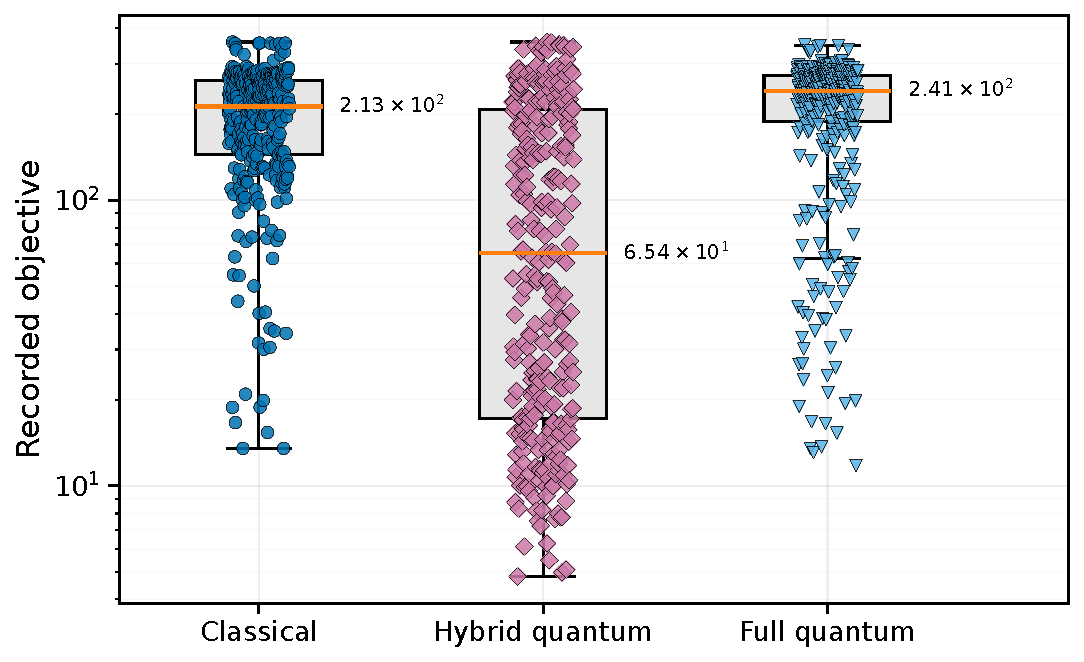
\includegraphics[width=0.86\textwidth]{../../analysis/optuna_tidal_test_hard_three_family_reupload/figures/optuna_model_family_comparison.pdf}
\caption{Tide: scoring loss by family. The annotation gives the median.}
\label{fig:tide-family}
\end{figure}

Figure~\ref{fig:tide-pareto} shows how the families compare across
parameter counts. Below about 100 parameters,
almost all hybrid and full-quantum models alternate along the front. At larger
parameter counts, through the lowest-loss region, the front consists of
hybrid models. Classical trials remain in the cloud above it.

\begin{figure}[ht]
\centering
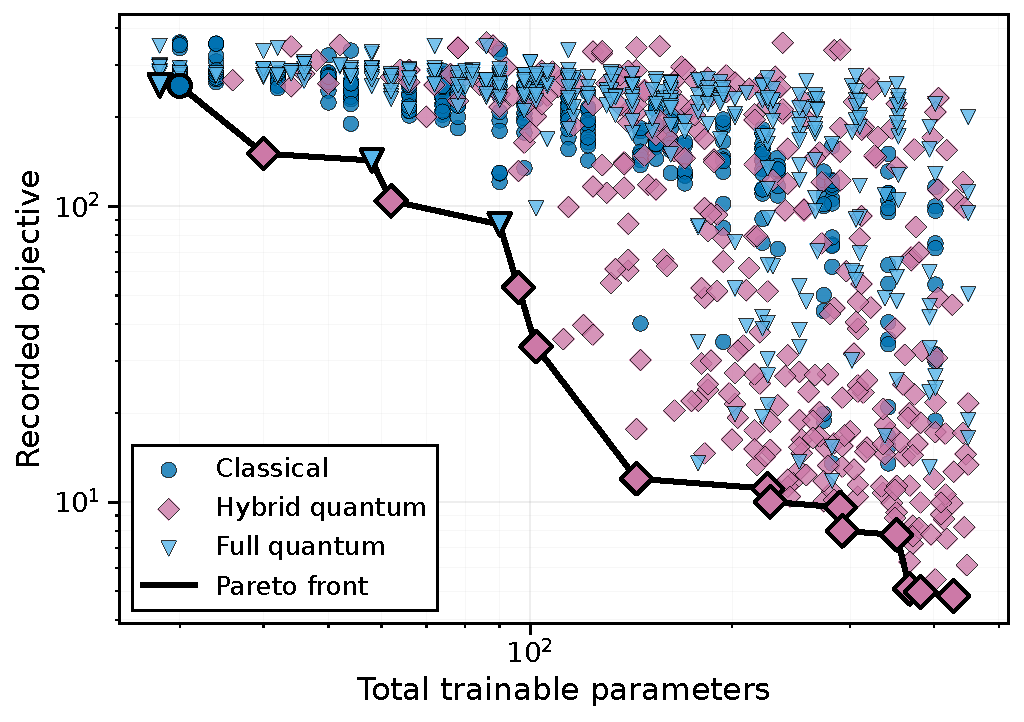
\includegraphics[width=0.86\textwidth]{../../analysis/optuna_tidal_test_hard_three_family_reupload/figures/optuna_pareto_front.pdf}
\caption{Tide: scoring loss against parameter count. Large markers
show the Pareto front; hybrid models occupy its low-loss end.}
\label{fig:tide-pareto}
\end{figure}

Retraining the winning hybrid reproduces the three-period tide
(Figure~\ref{fig:tide-fields}). Relative \(L_2\) errors are
\(2.88\times 10^{-2}\) for elevation and \(7.52\times 10^{-2}\) for
velocity. The largest elevation error occurs near the closed end during
the first period. The largest velocity error occurs in the interior
during that period. Both errors are smaller during the later periods.
For this smooth target, the architecture with the lowest scoring loss
also provides a recognizable solution of the initial-boundary-value
problem.

\begin{figure}[ht]
\centering
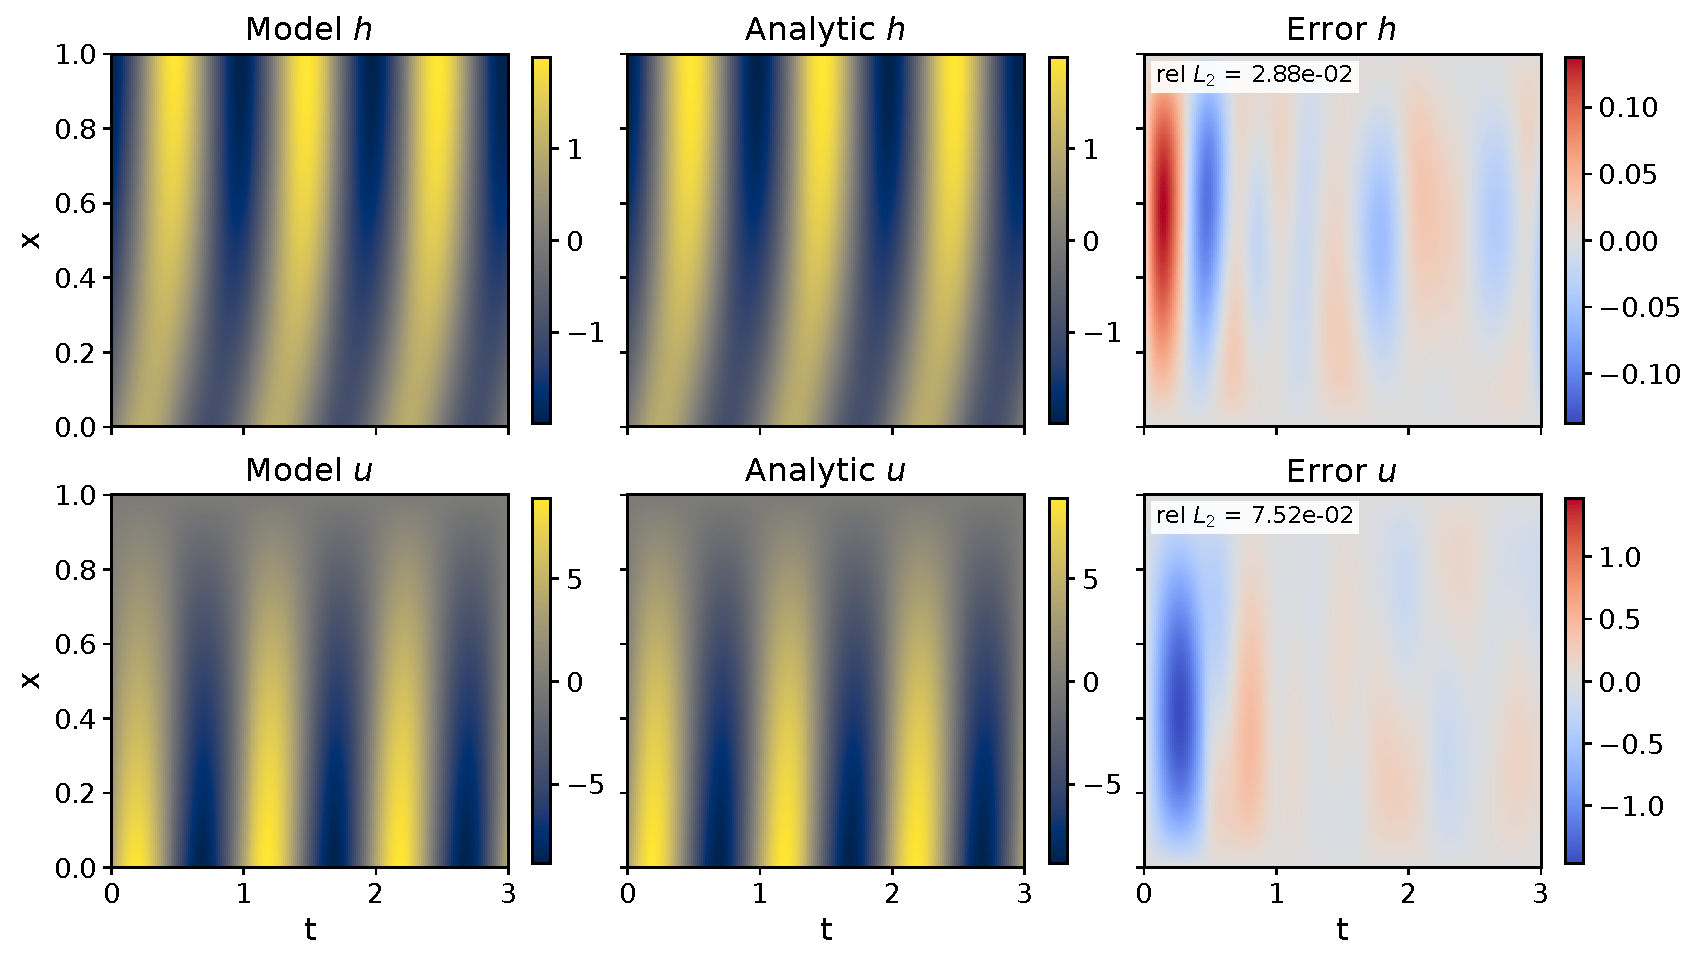
\includegraphics[width=0.98\textwidth]{../../analysis/optuna_tidal_test_hard_three_family_reupload/figures/model_vs_analytic.pdf}
\caption{Retrained tidal hybrid and exact solution. Time is measured in
tidal periods. The right column shows pointwise error.}
\label{fig:tide-fields}
\end{figure}

\subsection{Wet-bed dam break}
\label{sec:results-dam}

The dam-break study uses soft constraints, so its scoring loss includes
the equation residuals in~\eqref{eq:dambreak} and the weighted initial
and wall penalties. The score is evaluated on a \(101\times 41\)
lattice. The search completed 677 trials: 238 classical, 207 hybrid,
and 232 full-quantum.

\begin{table}[ht]
\centering
\caption{Best dam-break model in each family. Mass and momentum are
equation residuals; initial and boundary are weighted penalties.}
\label{tab:dam-best}
{\footnotesize
\begin{tabular}{lrrrrrr}
\hline
Family & Parameters & Mass & Momentum & Initial & Boundary & Loss \\
\hline
Classical & 234 & 0.00920 & 0.0123 & 0.113 & 0.00849 & 0.143 \\
Hybrid & 368 & 0.00816 & 0.0119 & 0.102 & 0.00643 & 0.128 \\
Full quantum & 450 & 0.00757 & 0.00650 & 0.131 & 0.00488 & 0.150 \\
\hline
\end{tabular}}
\end{table}

The hybrid model again has the lowest total loss: it has width 5, depth
4, four qubits, two circuit layers, and 368 parameters
(Table~\ref{tab:dam-best}). Its loss is 10\% lower than that of the
best classical model, but the advantage does not come from lower
equation residuals alone. The hybrid's initial-condition penalty is
\(0.102\), out of a total loss of \(0.128\). Across the three best
models, mass and momentum residuals range from \(0.006\) to \(0.013\).
The best full-quantum model has the smallest equation residuals of the
three, but its larger initial-condition penalty places it third by total
loss.

Median losses are \(0.410\) for classical trials, \(0.517\) for hybrid
trials, and \(0.406\) for full-quantum trials
(Figure~\ref{fig:dam-family}). The hybrid median is higher than the
other two. Full-quantum trials extend to a loss of \(73.4\), whereas
classical and hybrid trials remain below \(1.33\) and \(1.26\),
respectively.

\begin{figure}[ht]
\centering
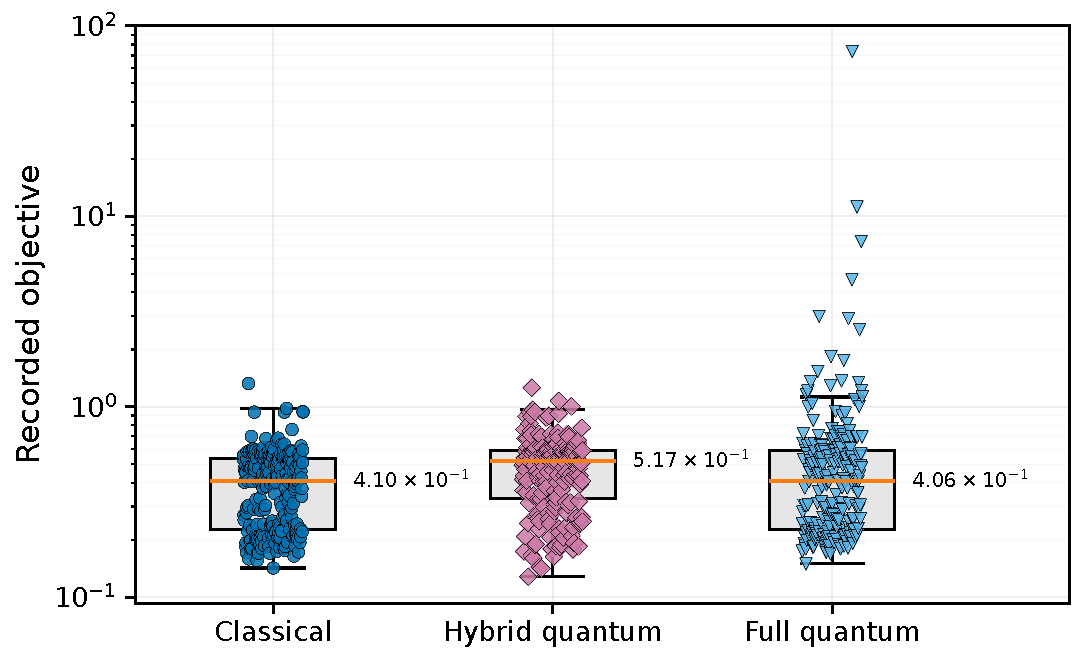
\includegraphics[width=0.86\textwidth]{../../analysis/optuna_dam_break_step/figures/optuna_model_family_comparison.pdf}
\caption{Dam break: scoring loss by family. The hybrid median is higher
than the classical and full-quantum medians.}
\label{fig:dam-family}
\end{figure}

Figure~\ref{fig:dam-pareto} shows why the single winning hybrid does not
make the hybrid family the best overall representation for this
problem. Below about 100 parameters, classical and full-quantum models
share the front. At larger parameter counts, the front consists of a
hybrid model at 168 parameters, classical models at 194 and 234
parameters, and the hybrid winner at 368 parameters. The winning hybrid
is the only completed trial with a loss below that of the best
classical model.

\begin{figure}[ht]
\centering
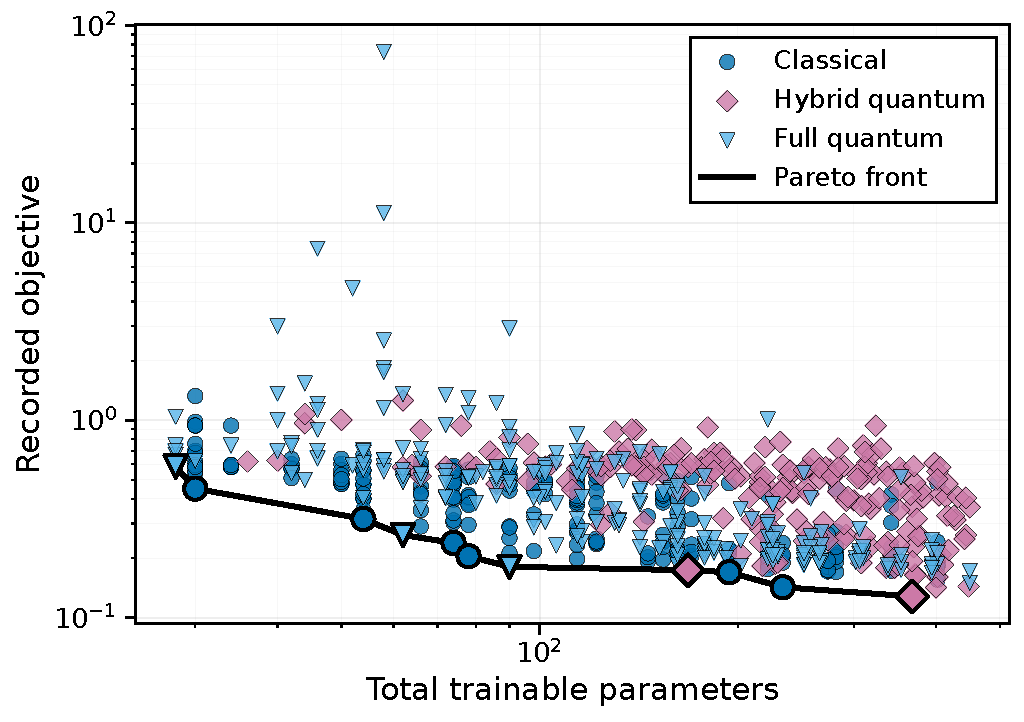
\includegraphics[width=0.86\textwidth]{../../analysis/optuna_dam_break_step/figures/optuna_pareto_front.pdf}
\caption{Dam break: scoring loss against parameter count. Large markers
show the Pareto front. One hybrid trial has lower loss than the best
classical trial.}
\label{fig:dam-pareto}
\end{figure}

The retrained hybrid places the rarefaction and shock in the correct
regions of the \((x,t)\) plane (Figure~\ref{fig:dam-fields}). Relative
\(L_2\) errors are \(3.43\times 10^{-2}\) for depth and
\(1.78\times 10^{-1}\) for velocity. The pointwise error follows the
two wave fronts. The network represents the jump in the exact solution
as a steep but continuous transition. Velocity error is larger than
depth error because the exact velocity is discontinuous across the
shock and changes abruptly through the rarefaction. Away from the
fronts, the depth plateau and still-water region remain close to the
reference.

\begin{figure}[ht]
\centering
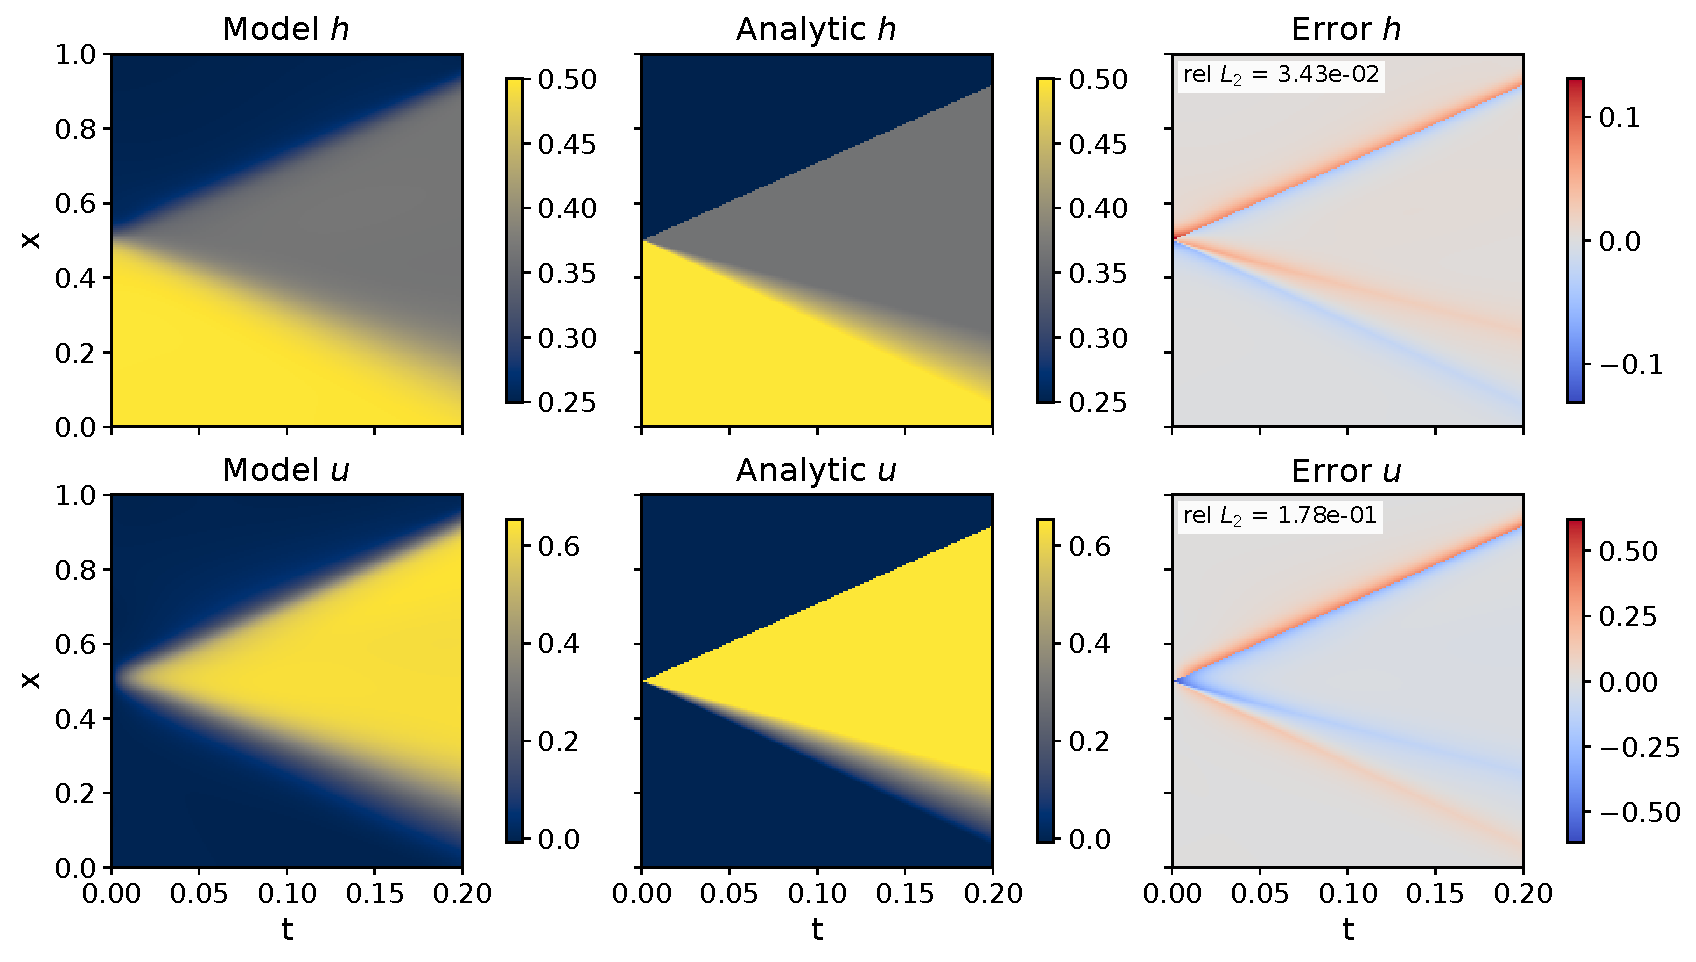
\includegraphics[width=0.98\textwidth]{../../analysis/optuna_dam_break_step/figures/model_vs_analytic.pdf}
\caption{Retrained dam-break hybrid and the Stoker solution. Time is
measured in seconds and \(x\) in meters. Error is concentrated along
the smoothed wave fronts.}
\label{fig:dam-fields}
\end{figure}

\subsection{Steady eddy lattice}
\label{sec:results-eddy}

The eddy study enforces the slip-wall traces with a hard constraint, so
its scoring loss is the sum of the three steady residuals
in~\eqref{eq:eddies}. The score is evaluated on a \(96\times 96\)
lattice. The search completed 514 trials: 183 classical, 151 hybrid,
and 180 full-quantum. The target is the \((m,n)=(7,4)\) lattice.

\begin{table}[ht]
\centering
\caption{Best eddy-lattice model in each family. Loss is the sum of
the mass residual and both momentum residuals.}
\label{tab:eddy-best}
\begin{tabular}{lrrrrr}
\hline
Family & Width & Depth & Qubits & Parameters & Loss \\
\hline
Classical & 5 & 6 & --- & 513 & 24.51 \\
Hybrid & 5 & 2 & 5 & 558 & 4.012 \\
Full quantum & --- & --- & 4 & 339 & 13.91 \\
\hline
\end{tabular}
\end{table}

The lowest loss comes from a hybrid model with width 5, depth 2, five
qubits, and five circuit layers (Table~\ref{tab:eddy-best}). Its
scoring loss of \(4.01\) is 84\% below the best classical loss of
\(24.5\). The best full-quantum model, with four qubits and eight
layers, lies between them: its loss is \(13.9\), with 339 parameters.
The residual breakdown follows the same ordering. The winning hybrid
has mass and momentum contributions of \(2.32\) and \(1.69\). The best
full-quantum model has contributions of \(7.51\) and \(6.40\), while
the best classical model has contributions of \(8.80\) and \(15.7\).

The family medians are closer than the best-model losses: 69.2 for
classical trials, 52.2 for hybrid trials, and 60.5 for full-quantum
trials (Figure~\ref{fig:eddy-family}). The hybrid interquartile range
overlaps those of the other families, while hybrid trials alone reach
losses near four.

\begin{figure}[ht]
\centering
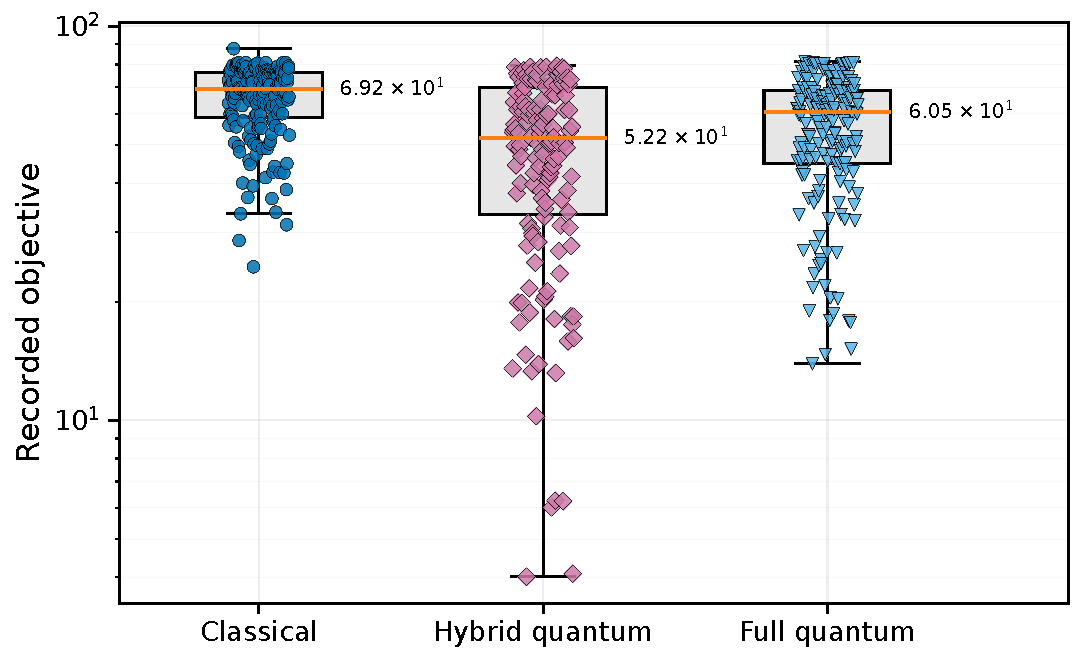
\includegraphics[width=0.86\textwidth]{../../analysis/optuna_steady_eddies_hard_three_family/figures/optuna_model_family_comparison.pdf}
\caption{Eddy lattice: scoring loss by family. The annotation gives
the median. Hybrid trials reach the lowest losses.}
\label{fig:eddy-family}
\end{figure}

Figure~\ref{fig:eddy-pareto} shows how the two quantum families occupy
different parts of the front. Below about 340 parameters, most of the
front consists of full-quantum models, with hybrid models interleaved.
From 435 parameters through the 558-parameter winner, the front
consists of hybrid models. Classical trials remain above the
low-loss end. Within the searched parameter range, hybrid models reach
the lowest losses, while full-quantum models occupy most of the
low-parameter region.

\begin{figure}[ht]
\centering
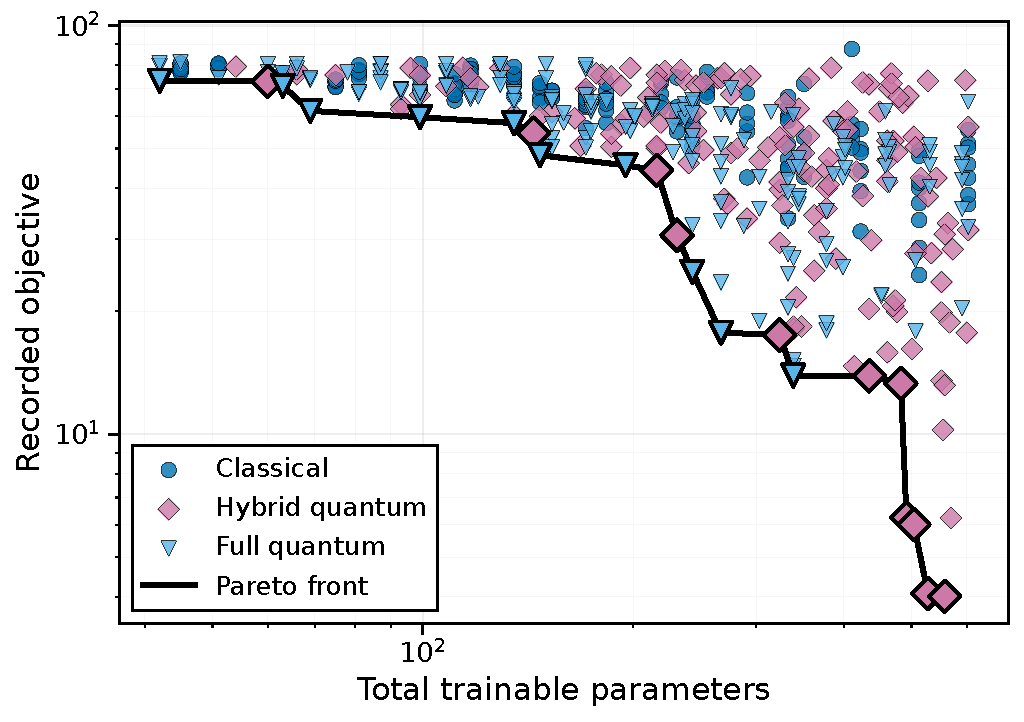
\includegraphics[width=0.86\textwidth]{../../analysis/optuna_steady_eddies_hard_three_family/figures/optuna_pareto_front.pdf}
\caption{Eddy lattice: scoring loss against parameter count. Large
markers show the Pareto front. Full-quantum models occupy most of the
low-parameter region, while hybrid models occupy the low-loss region.}
\label{fig:eddy-pareto}
\end{figure}

Retraining the winning hybrid does not produce an accurate velocity
field, despite its low scoring loss (Figure~\ref{fig:eddy-fields}).
The model captures the depth pattern of the lattice, with a relative
\(L_2\) error of \(1.25\times 10^{-2}\), but it does not capture the
velocity fields. Their relative \(L_2\) errors are \(1.21\) for \(u\)
and \(1.30\) for \(v\), both larger than the corresponding exact
fields. The analytic velocity contains the small-scale sign changes
of the \((7,4)\) mode pair; the retrained model instead produces a
smooth field with a few broad extrema. Because the hard constraint
builds the exact boundary traces into the output, this discrepancy
arises in the interior. The study's lowest scoring loss remains of
order four rather than approaching zero. The field comparison shows
that this residual loss did not ensure that the oscillatory velocity
structure was resolved.

\begin{figure}[ht]
\centering
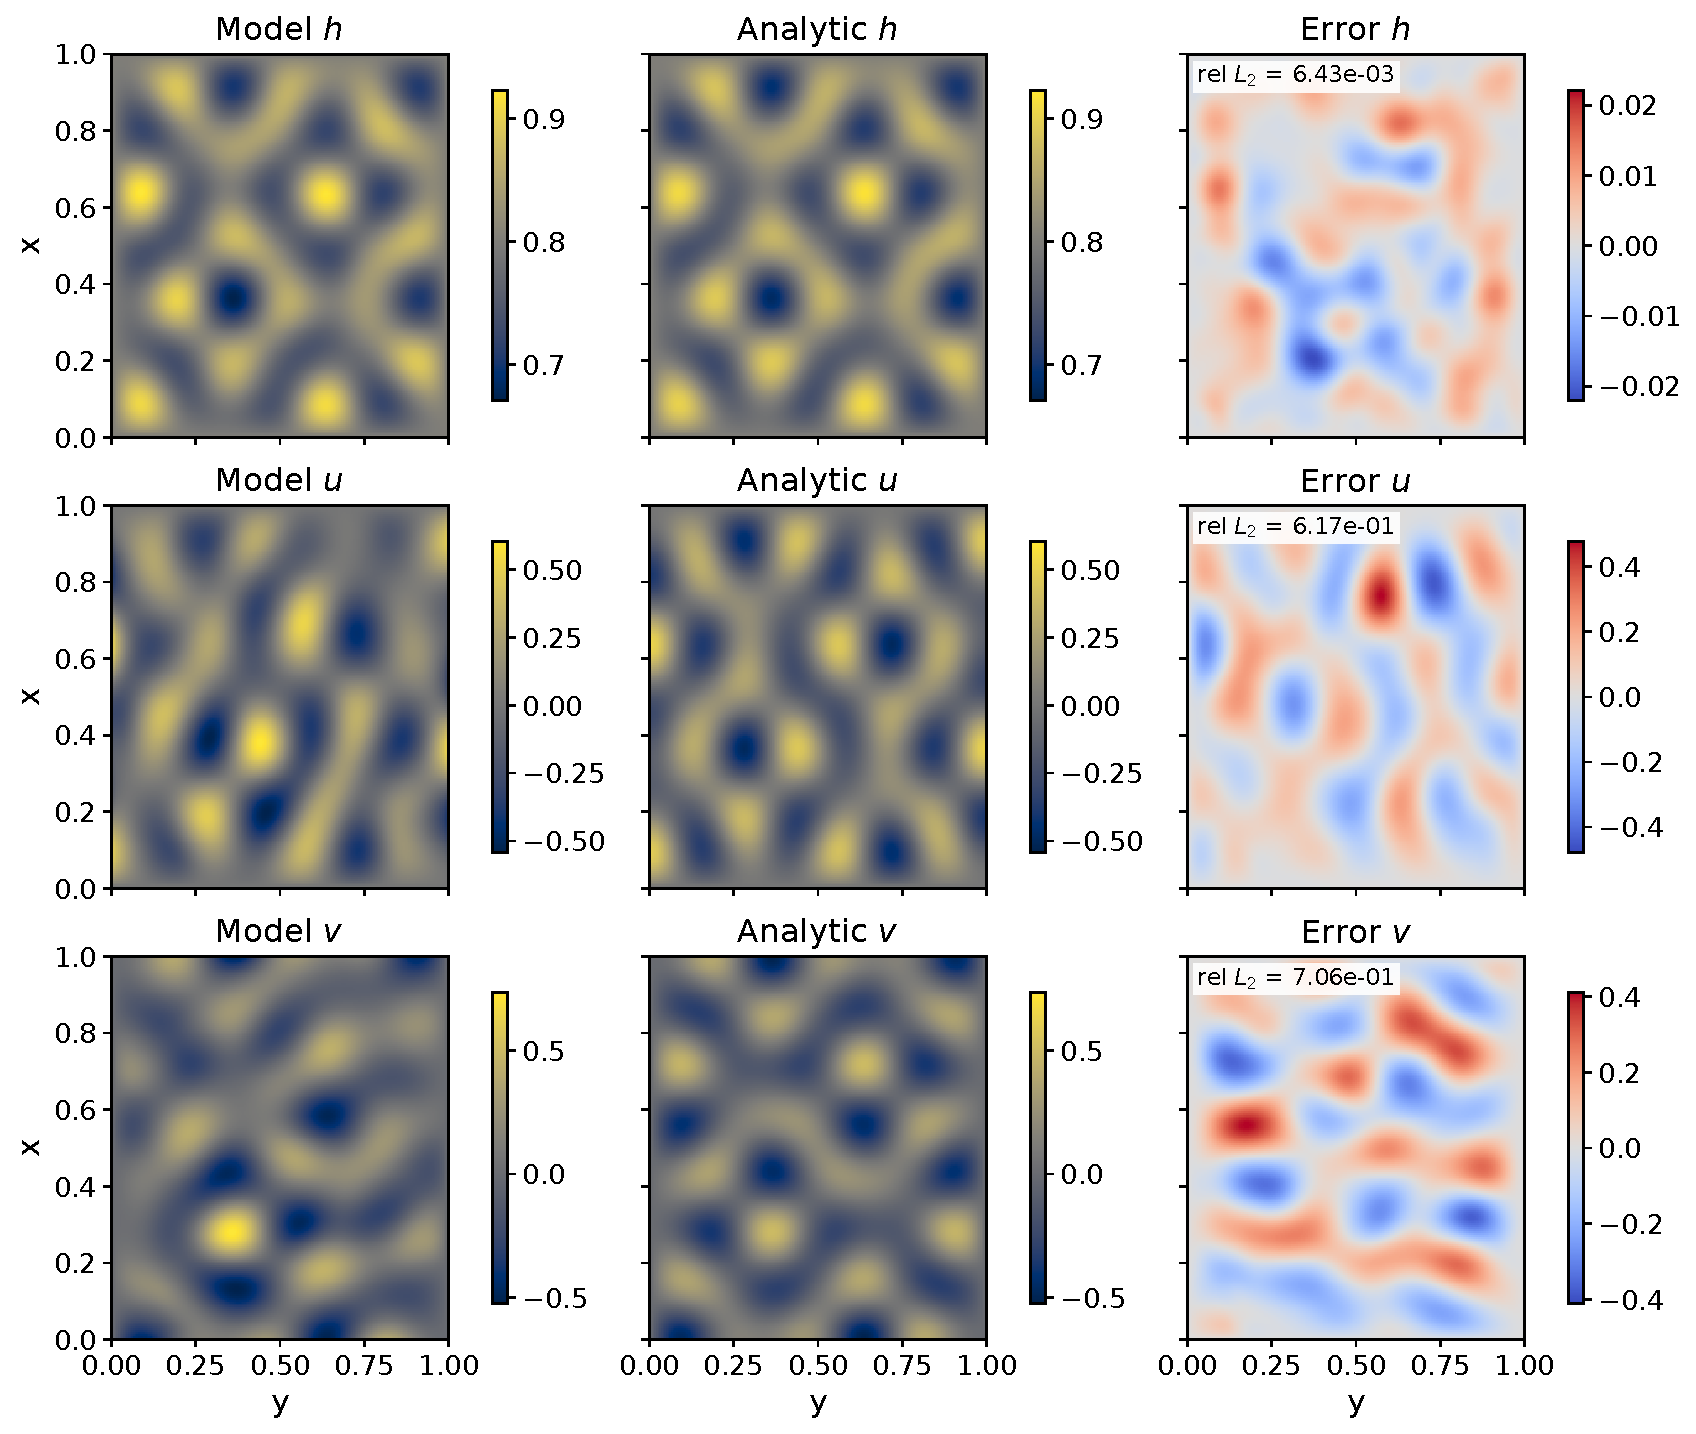
\includegraphics[width=0.92\textwidth]{../../analysis/optuna_steady_eddies_hard_three_family/figures/model_vs_analytic.pdf}
\caption{Eddy hybrid and exact solution. The model captures the depth
lattice, but the velocity error exceeds the magnitude of the exact
velocity.}
\label{fig:eddy-fields}
\end{figure}


\chapter{Conclusion}
\label{sec:conclusion}

The three studies use the same search space and ranking rule, yet produce different results for each solution class.

For the linear tide, the hybrid circuit is the strongest representation within the search space. Hybrid models occupy the low-loss end of the Pareto front, and the winning model lowers both equation residuals relative to the best classical and full-quantum models. When retrained, it follows the analytic wave with a few percent relative error in elevation and less than ten percent in velocity.

For the wet-bed dam break, the classical trunk is already competitive. Classical models remain on the Pareto front through the lowest classical loss, and only one hybrid trial improves on it. The best hybrid’s total loss is about ten percent lower, with most of that margin coming from its smaller initial-condition penalty. The equation residuals of the three best models are similar, and the best full-quantum model has the smallest combined equation residual. The retrained hybrid places the rarefaction and shock correctly but smooths both fronts. Within this search, the circuit does not establish a clear advantage for a discontinuous shallow-water solution.

For the steady eddy lattice, scoring loss and solution error diverge. Hybrid models reach the lowest losses, while full-quantum models occupy much of the low-parameter region of the Pareto front. The retrained hybrid captures the depth lattice but misses the velocity lattice. The physics-informed loss selected the architecture; it did not certify its velocity field.

These findings are bounded by the search space. Classical trunks have at most five units in each of at most seven hidden layers. Quantum circuits are evaluated with a noiseless statevector simulator and use at most eight qubits and eight layers. The results compare representations within these limits; they do not compare against unrestricted classical networks or demonstrate quantum computational advantage. Within the tested range, hybrid corrections most often reach the lowest scoring losses, while full-quantum circuits compete at the smallest parameter counts. Agreement with the exact fields must still be assessed after ranking by loss; it cannot be inferred from that ranking alone.

\bibliographystyle{plainnat}
\bibliography{hpinn_sw}

\end{document}
